\chapter{Introduction}

This introductory chapter is organized in three sections; the first section on background justification will provide selected context necessary to justify the need for research on maritime communities, including the prior claims in the literature that attest to “Ship’s language” as a distinct variety and some of the reasons why this subject has been neglected in the scholarship of dialectology and contact linguistics. The second section on the scope and purpose of the research will provide the hypothesis, research aims and five research questions formulated to investigate characteristic features of sailors’ speech in the early English \isi{colonial period}. It will also give selected details on the ideological and academic context that has influenced my own thought process regarding the focus of this study. The last section presents the methodological framework of the study, with details on the \isi{research design} and a description of the \isi{corpus} with details on the three subsections of documentation used. This introduction ends with a brief outline of each of the subsequent chapter’s contents.



\section{{Background} {justification} }%1.1



\subsection{{The} {need} {for} {research} {on} {maritime} {communities}}%1.1.1



We live in a world so interconnected by air travel, media and online networks that we rarely consider the importance of maritime travel or those who depended upon it in an age before we physically and digitally took to the skies. Yet maritime communities were profuse and critical to the development of the early European colonies during an age of expansion that set off dynamic and often unpredictable changes throughout the known world. Yet what we think we know about the culture and customs of the people who inhabited these communities can owe less to scholarship than to popular stereotype. 



At the center of diverse and multicultural maritime communities were a host of men, women and children who lived and worked predominantly at sea yet who are remembered through the stereotype of the able \isi{seaman} in his mid-twenties who hauled ropes and drank grog serving on a large naval ship of the line. Rarely do we consider the complexities of the real maritime communities that were composed of ranked strata in a three-tier class system. First in command, a small upper-class of commissioned and warrant officers included ranks such as admiral, captain, lieutenants, master, purser, surgeon, boatswain, gunner, and carpenter. Second in line, a moderate middle class of petty officers and militia included ranks such as armorer, cook, gunsmith, sailmaker, schoolmaster, master-at-arms, midshipmen, coxswain, quartermaster, and gunners’ mates, and soldiers. Lastly, a majority of lower class workers included ranks such as able seamen, ordinary seamen, landsmen, servants, and boys. And, in addition to these officially recognized \isi{crew}, a range of largely undocumented transient passengers, workers, servants, wives, and slaves frequently accompanied the ship for short legs and entire voyages. Yet, these people were not wage-earners and so their presence is often hidden by the official records. Thus, what we think we know about the people who inhabited maritime worlds fails to incorporate the complex realities of these working and living spaces.  



Further to our limited recognition of the people who made up the communities of large ships, we also fail to recognize the range of vessels that hosted different types of maritime communities. The shipping lanes of the seventeenth and early eighteenth centuries were replete not only with large naval and \isi{merchant} vessels with the type of social hierarchy detailed above, including the caravel, carrack, galleass, galleon and hulk, but also a myriad of mid-to-small scale vessels. These smaller vessels ranged from the mid-sized barge, barque, brigandine, cromster, frigate and pinnacle, used for speed and maneuverability in long-range voyages, to the small-scale flute, flyboat, galley, hoy and shallop, used not only for support work such as supply and boarding enemy vessels, but also surprisingly long-range but small-scale trade operations designed to evade customs regulations and hence also documentation (\citealt{Bicheno2012}.) These smaller vessels were frequently employed in trade, but also made voyages of exploration, colonization, political expansion, passenger transit, salvage, supply and smuggling (\citealt{Jarvis2010}.) And these classifications were not mutually exclusive as a simplified historical glance has encouraged us to believe. Furthermore, all of these vessels likely had an on-board community that was unique to the size and requirements of the cargo space, rigging, defense system, and navigational capacities. By failing to recognize these vessels and their unique communities in our largely simplistic historical representations, we cannot hope to understand the cultures of the people who worked and lived aboard them and who were critical agents in the expansion of European colonial regimes. 



\subsection{{Ship’s} {language} {as} {a} {distinct} {variety}}%1.1.2



The linguistic focus of this research stems from the claim there is a distinct “Ship English” that was spoken by British sailors in the early colonial context (the term coined by \citealt{Hancock1976}: 33.) However, long before the relevance of \isi{maritime language} use was championed by Hancock in his theories on \isi{creole genesis} (\citealt{Hancock1972}; 1976; 1986; 1988,) the idea that sailors used distinct language forms was attested to in a host of lexical compilations and user manuals. \citealt{In1627}, Captain John Smith published \textit{Smith’s Sea Grammar} in which he gives “expositions of all the most difficult words seldome used but amongst sea men” (\citealt{Smith1968} [1627,] §Table of Contents) and offers explanations and translations for “the language both of ships and Seas” (\citealt{Smith1968}, §In Authorem.) This \textit{Sea Grammar}, despite its name, was not so much a linguistic analysis as a handbook divided into content-specific chapters about how to manage oneself at sea, for which language skills were considered essential. The fact that this book was reprinted in 1627 1636 1641 and 1653 attests not only to the usefulness but also the popularity of its contents, a trend echoed by the subsequent publication of Manwayring’s \textit{The Sea-Man’s Dictionary,} in 1644, reprinted in 1666 1667 1670 and 1675-82. 



The concept of a “Sea Grammar” was not restricted to English. Not long after Smith’s manual was published in English, publications about sailors’ talk in French appear in the mid-\isi{seventeenth century} such as Cleirac’s \textit{Explication des Termes de Marine...} (1639 reprinted 1647 and 1660) and the anonymous broadsheets \textit{Déclaration des Noms Propres des Piàces de Bois et Autres Pièces Nécessaires Tant à la Construction des Navires de Guerre …}(1657) and \textit{Termes Desquels on Use sur Mer dans le Parler…}(1681 reprinted in 1693) followed by Desroches’s \textit{Dictionnaire des Termes Propres de Marine...} (1687.) The \isi{late seventeenth century} also saw the Dutch publication \textit{W. à Winschootens Seeman…} (\citealt{Winschooten1681},) the Spanish publication by Fernández de Gamboa \textit{Vocabulario de los Nombres que Usan la Gente de Mar} (1698,) and the anonymous publication \textit{Vocabulario Marítimo y Explicacion de los Más Principales Vocablos} (1696 reprinted 1698.) Hence, the concept of a distinct variety that was unique to maritime communities was not an isolated phenomenon around the trading routes of the British Isles but a common characteristic of maritime communities with enough salience to have grammars published as early as the \isi{seventeenth century} in at least four European languages. 



Since these early popular publications of the \isi{seventeenth century} a host of other manuscripts, pamphlets and books targeted those readers with an occupational or personal interest in life and language at sea. These publications were invariably composed of lexical entries, as the titles reflect, e.g., Monke’s \textit{Vocabulary of Sea Phrases} (1799) and Neumann’s \textit{Marine Pocket-Dictionary} (1799.) And this focus on sailors’ lexicon has continued up until the more recent publication of works like Jeans’s \textit{Dictionary of Everyday Words and Phrases Derived from the S}\textit{ea} (1993) and the web-based reference work \textit{Seatalk, The Dictionary of English Nautical Language} (\citealt{MacKenzie2005}.) Although many of these lexicons are aimed at those with an occupational or historical interest, there are also a host of publications that cater to general interest and entertainment markets, such as \textit{The Pirate Primer: Mastering the Language of Swashbucklers and Rogues} (\citealt{Choundas2007}.) Yet, despite the many publications that cater to different reader demographics, nearly all compose word-lists in the style of dictionary entries and perpetuate the belief that what made - and continues to make - \isi{maritime language} different and interesting is its use of particular words, suggesting that the variety is a technical jargon. 



\subsection{{A} {neglected} {subject} {in} {academia}}%1.1.3



Despite the rush of titles aimed at readers with an occupational interest in maritime use of language, very few academic papers have investigated the complexities of Ship English beyond its lexicon.  The dearth of academic studies of \isi{maritime language} use may reflect the fact that investigations would have be inter- and intra-disciplinary: the necessary archival research might be better suited to a historian; the identification of correlating language forms in literary representations more suited to a literature specialist; the analysis of how maritime communities functioned more suited to a researcher in maritime studies; and the understanding of interconnectivity more appropriate for a researcher in Atlantic studies. Even within the discipline of linguistics: the suggestion that Ship English is a language variety alludes to theories of dialectology; the idea that it was formed by communication among multilingual communities necessarily involves theories of \isi{pidgin} and \isi{creole} studies; and the belief that the composition of the community directed \isi{language change} involves theories of sociolinguistics. I do not suggest that the study of Ship English is unique in its complexities for the potential researcher, but these challenges, coupled with the fact that there is little groundwork on this subject upon which to base new studies, potentially impede investigations from being undertaken. 



  In addition to the theoretical complexities, a potential researcher is faced with a host of practical challenges. Even for the workers who left a record of their presence on the ships (and many didn’t) they were a transient and demographically complex group to determine (\citealt{AdkinsAdkins2008}: 176-177; \citealt{Fusaro2015}: 8.) Particularly in the period of early \isi{colonial expansion}, workers in the maritime world were often not required to provide any kind of information to officials such as their age, place of origin, social status or language abilities that a researcher could use to determine demographics (\citealt{Litter1999}: 125 \& 191,) nor were many of these workers obliged to remain in the same service vessel for a long period of time. It was entirely possible that they moved from vessel to vessel and port to port following the opportunities that appeared to be most beneficial at any given time. Sailors might remain working on one trade route and therefore spend time in its associated ports for years, or they might be constantly changing trade routes, locations, and port regions in addition to time potentially spent out of work in one place - whether that be a home port or a foreign location. Furthermore, studies indicate that as much as one third of shipping activity may have escaped the official records (\citealt{Cook2005}: 15.) It is therefore extremely difficult to determine probable regional influences on sailors’ transient populations or to locate them in geographical models of \isi{dialect} areas.



Practical difficulties for the researcher are compounded by the recognition that most seventeenth and \isi{eighteenth century} seamen were illiterate \citep[167]{Kelly2006} and therefore were unlikely to have left any written evidence of their speech. Even in cases where hand-written records existed, they may not have made it into the public record, for example, in cases of piracy, documentation was often burned, destroyed, or thrown overboard. The few records of authentic sailors’ writing that we do have are often so formulaic and dry (e.g., logbook entries,) so fraught with literary overtones (e.g., travel journals,) or so affected by prescribed stylistic written forms (e.g., letters from the captain) that they are considered poor samples of authentic speech. Furthermore, even if the researcher is lucky enough to find preserved writing samples reflective of authentic speech the script is often extremely difficult to decipher as it was composed in Early Modern English prose in an age before consistent standardized spelling and \isi{punctuation}, and very often with nearly illegible handwriting owing to individual penmanship preferences, a moving vessel, or the unpracticed hand of its author. Yet even if the words \textit{are} legible, the researcher also needs to recognize and interpret maritime abbreviations, acronyms and symbols before the meaning of a sentence can be analyzed for its syntax and grammatical structures. In short, designing an interdisciplinary research methodology that integrates the theories and practices of a range of linguistic sub-disciplines and mitigates the potential challenges of data collection and analysis with no tested model upon which to base a research strategy likely discourages even the most interested scholar. 



Despite these significant methodological difficulties, a few scholars have attempted to break ground on the neglected subject of Ship English beyond its lexicon. Two notable studies are \citeapo{Matthews1935} monograph on sailors’ pronunciation in the second half of the \isi{seventeenth century} based on phonetic spellings in ships’ logbooks; and Bailey and \citegen{Ross1988} article on the morphosyntactic features of Ship English that focuses on evidence of variation in \isi{tense marking} and the \isi{copula}, also based primarily on logbooks. Yet, to my knowledge, there have been no new studies of phonological, morphological, syntactic, or discourse-level variation in Ship English since Bailey and Ross’s last article in the late 1980s and no studies using a \isi{corpus} that extends beyond logbooks and selected papers of the (English) Royal African Company. In response to the academic hesitation on this subject, this book has been conceptualized to continue the valuable earlier work of Matthews, Bailey and Ross and to motivate renewed interest in the subject.  



\section{{Scope} {and} {purpose} {of} {the} {research}  }%1.2



\subsection{{Hypothesis,} {research} {aims} {and} {questions}}%1.2.1



This book presents evidence in support of the hypothesis that Ship English of the early Atlantic \isi{colonial period} (determined roughly as the period between 1620 and 1750) was a distinct variety with characteristic features. Its two principal aims are firstly, to outline the socio-demographics of the maritime communities and examine how variant linguistic features may have developed and spread among these communities, and secondly, to generate baseline data on the characteristic features of Ship English. These aims will be addressed through five research questions that relate to establishing demographic data on sailors, collating sociolinguistic data that attest to how their speech communities functioned, and identifying characteristic features of their speech at the word, phrase, sentence, and discourse levels. The five research questions, each of which is discussed in a dedicated chapter, are as follows:


\begin{itemize}
\item Who were the English-speaking sailors of the early colonial Caribbean?
\item How did sailors’ speech communities function?
\item What are the salient markers of sailors’ speech in \isi{noun} phrases?
\item What are the salient markers of sailors’ speech in \isi{verb} phrases?
\item What variation characterizes sailors’ speech in syntax and discourse?
\end{itemize}

Anticipated findings will not only substantiate Bailey and Ross’s claim that there is a distinct type of English that was spoken by sailors during the period of early English \isi{colonial expansion} (1988: 194) but also provide baseline data that may serve as an entry point for scholars to integrate this language variety into the discourse on \isi{dialect} variation and \isi{language contact} in the early \isi{colonial period}. 


\begin{itemize}
\item 
\begin{itemize}
\item 
\begin{itemize}
\item \textbf{Ideological} \textbf{and} \textbf{academic} \textbf{context}
\end{itemize}
\end{itemize}
\end{itemize}

It is perhaps important to explain that I came to the subject of Ship English through studies in Caribbean languages at the University of Puerto Rico, Rio Piedras campus. I formulated the \isi{research design} and focus of the study as part of my doctoral degree in the literature and languages of the English-speaking Caribbean with a specialization in linguistics, and the final research on which this book is based formed the backbone of my doctoral dissertation. My academic preparation in Caribbean linguistics exposed me to theories of languages in contact and the formation of trade pidgins and new \isi{creole} languages. I was intrigued by theories of universalism (e.g., \citealt{MuyskenSmith1986}; \citealt{McWhorter2011}) and scholarship on pan-Caribbean language forms (e.g., \citealt{Allsopp2003}; Faraclas, Corum, Arrindell, \& \citealt{Ourdy2012}.) I have been additionally motivated in my research endeavors by the late Mervyn Alleyne, whose work on sociolinguistics, creoles and dialects of the Caribbean has driven a whole generation of scholars fortunate enough to study under his tutelage. With an interest in \isi{creole} universals and \isi{historical dialectology}, I was fortunate enough to receive guidance from historical linguist Ann Albuyeh, creolist Nicholas Faraclas, and literature specialist Michael Sharp in the development of my research plans, all of whom composed the academic committee of my doctoral research, as did Mervyn Alleyne until his passing in November of 2016. Considering this academic context, it is perhaps no surprise that I came to the subject of Ship English through \isi{creole} studies and I envision the intellectual merit of the findings in terms of how scholars may integrate this variety in future studies of languages in contact.



Yet, despite the \isi{creole} focus in the academic context of this research, I would like to stress that I do not present these findings in support of any one theory of \isi{creole} linguistics. Specifically, I do not propose that these findings promote either side of the polemic substrate-\isi{superstrate} debate nor promote any specific theory of \isi{language transfer}, \isi{dialect formation} nor universalism, although I recognize the potential for the findings to be applied to such subjects. My intention differs from previous assertions that a potential type of language spoken on ships influenced \isi{creole} development (e.g., \citealt{Reinecke1938}; \citealt{Hancock1972}; 1976) and instead claims to gather baseline data that substantiates the fundamental claim that Ship English of the early \isi{colonial period} was a distinct variety. As an investigation into the characteristics of Ship English as a distinct variety, this study would therefore be more suited to \isi{dialect} studies than creolistics. However, given the implications of the findings in light of \isi{creole} theories, I will clarify my own position and highlight potential applications of the findings for different schools of thought in the last chapter containing conclusions and implications. 



\section{{Methodological} {framework}}%1.3



\subsection{{Research} {design}}%1.3.1



A mixed methods triangulation design was employed in this research, selected to suit my intention “to directly compare and contrast quantitative statistical results with qualitative findings or to validate or expand quantitative results with qualitative data” (Creswell \& Plano \citealt{Clark2007}: 62.) The specific triangulation model used was the traditional convergence model in which a researcher collects and analyzes both qualitative and quantitative data concurrently and converges the data at the stage of comparison and contrast (see \figref{fig:key:1}.1, based on Creswell \& Plano \citealt{Clark2007})


\begin{figure}
 
%%please move the includegraphics inside the {figure} environment
%%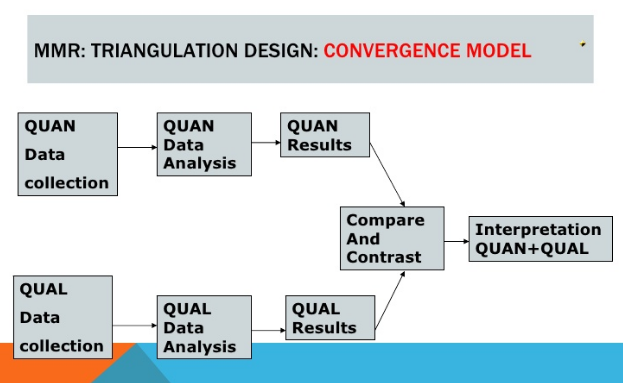
\includegraphics[width=\textwidth]{figures/delgado-img1.png}

\caption{\label{fig:key:1}.1}: A mixed methods triangulation research design using the convergence model, by courtesy of Gustavo Daniel Constantino and Slideshare.net, based on Creswell \& Plano \citealt{Clark2007}: 63 © 2012, Gustavo Daniel Constantino; used with permission. 
\end{figure}



The two main benefits of this triangulation convergence model are: firstly, its efficiency in that data types are collected simultaneously during one phase of the research plan; and secondly, its potential to mitigate the weaknesses of the quantitative component (e.g., limited sample size and authenticity of written representations) with the strengths of the qualitative component (e.g., salience and data on perceptual dialectology.) However, this model also has challenges, such as managing different sample sizes, comparing dissimilar data, and selecting differential evaluation methods for the data sets in a way that enables meaningful comparison and interpretation. An additional challenge of this model relates to the fact that none of the samples in the \isi{corpus} were collected for the specific purpose of the research objectives; they are all archival documents. I therefore had to consider the original intention and audience of the material alongside the content and acknowledge potential bias in my analysis. 



It is important to note that this triangulation convergence model was first pilot-tested and validated in a smaller study of sailors’ \isi{phonology} which I carried out in 2014. The pilot study focused on a linguistic cross-comparison of literary and historical data using standard statistical measures of correlation to determine general tendencies. Conclusions indicated significant points of comparison from which general phonological characteristics could be determined and findings were presented at the summer meeting of the Society for \isi{Pidgin} and \isi{Creole} Linguistics at the University of Graz, Austria, 7-9 \citealt{July2015} in a paper entitled ‘The reconstructed \isi{phonology} of \isi{seventeenth century} sailors’ speech.’



\subsection{{Description} {of} {the} {corpus}}%1.3.2



Data collection strategies were designed to target written representations of sailors’ speech that were prepared or published between the dates 1620 and 1750, and which prioritized documents that were composed by working mariners. Both quantitative and qualitative data were sourced from archived originals or copies of documents maintained in one of the eight archives I visited, see \tabref{tab:key:1}.1 for details of archives, locations and dates of access.


\begin{table}\begin{tabularx}{\textwidth}{XXX}
\lsptoprule

\textbf{Archive} & \textbf{Location} & \textbf{Month/Year} \textbf{visited}\\
Whim Archive & Frederiksted, St. Croix & \citealt{May2010}\\
National Archives of Trinidad and Tobago & Port of Spain, Trinidad & \citealt{July2012}\\
The \isi{Barbados} Department of Archives & St. James, \isi{Barbados} & \citealt{July2013}\\
\isi{Barbados} Museum and Historical Society & Bridgetown, \isi{Barbados} & \citealt{July2013}\\
Colección Josefina del Toro Fulladosa & San Juan, Puerto Rico & Jan, \citealt{Feb2014}\\
The National Archives & Kew, London, England & June, July, \citealt{Nov2015}\\
The \isi{Merseyside} Maritime Museum & \isi{Liverpool}, England & \citealt{July2015}\\
The National Maritime Museum & London, England & \citealt{November2015}\\
\lspbottomrule
\end{tabularx}

\caption{\label{tab:key:1}.1}: Archival resources accessed for research
\end{table}



The document \isi{corpus} for this research is divided into three subsets of data classified as 1) depositions, 2) hand-written records, and 3) material for public consumption. The first subset, described more specifically as written records of witness depositions taken during the 1620-1750 period in admiralty court sessions, composes the majority of the \isi{corpus}. Although the caveat remains that these are written accounts of spoken depositions, likely to have been written (and potentially interpreted) by a \isi{court clerk}, they do nonetheless remain the closest account of sailors’ spoken language available to a present-day researcher. Many of these depositions are also signed, initialed or somehow marked to show the speakers’ corroboration of the material therein contained after presumably having it read back to them or reading over the testimony themselves. The second substantial subset of hand-written records includes letters, receipts, log books and miscellaneous records attesting to personal grievances, vessel movements, manning and/or trade activities during the 1620-1750 period in and around the Atlantic. These documents, although they were composed in the written mode, are potentially the most accurate reflection of idiomatic \isi{language use}, however they are necessarily reflective of only those \isi{crew} members who were literate, and were also likely to have been composed following an accepted format or linguistic style customary or prescribed for the context of each document. The third and smallest subset of the \isi{corpus} was written for public consumption and includes material such as broadsheets of sea-shanties, journals prepared for publication, and contemporary literary representations. It is important to note that whilst the maritime representations of speech contained in these documents remain valid, they are also the most likely to have been heavily revised, adapted, and stereotypically presented for entertainment purposes. However, these representations form an important part of the \isi{corpus} as they potentially speak to perceptions of salience in sailors’ speech that a popular audience might readily recognize. 



The three subsets of data were collated and analyzed concurrently following the triangulation \isi{research design} detailed above, and the findings of each data set were used to corroborate findings in the others with the intention of motivating a comprehensive analysis in which the weakness of any one subset was mitigated by the strengths of the others. See \tabref{tab:key:1}.2 below for a summary of the characteristics of the \isi{corpus} subsets. 





\begin{table}
\caption{\label{tab:key:1}.2}: Characteristics of the corpus subsets 
\begin{tabularx}{\textwidth}{XXXX}
\lsptoprule

\textbf{Corpus} \textbf{subset} & \textbf{Description} & \textbf{Strengths} & \textbf{Weaknesses}\\
\textbf{1)} \textbf{Depositions}

Est. 60\% of \isi{corpus} & Written records of witness depositions taken during admiralty court sessions & Composed in spoken mode, corroborated by speaker and includes potentially illiterate sailors & Likely to have been written (interpreted) by a \isi{court clerk}\\
\textbf{2)} \textbf{Hand-written} \textbf{records}

Est. 30\% of \isi{corpus} & Letters, receipts, log books and misc. documents of personal grievances, vessel movements, manning, trade & First-hand writing, reflects idiomatic \isi{language use} & Reflective of literate \isi{crew} only and potentially composed with a prescribed style\\
\textbf{3)} \textbf{Material} \textbf{for} \textbf{public} \textbf{consumption}

Est. 10\% of \isi{corpus} & Published sea-shanties, journals, news items, literature, advertising & Shows perceptions of recognized salience in sailors’ speech & Interpreted, revised, adapted, and possibly stereotypical \\
\lspbottomrule
\end{tabularx}
\end{table}

\subsection{{Outline} {of} {each} {chapter’s} {contents}}%1.3.3



  The first two chapters serve to orient the reader in terms of the aims, the research methodology and the chosen subject of focus. In this Chapter 1: Introduction, I have justified the need for the research, established its scope and purpose, and given details about the \isi{research design} and \isi{corpus}. Chapter 2: Review of the Literature will summarize the intentions and findings of the few scholars who have identified and studied Ship English in addition to presenting some theories of dialectology and methodological approaches in historical linguistics relevant to the \isi{research design}. 



  The subsequent chapters 3 and 4 will have a socio-historical focus and respond to the first two of the research questions detailed above: Who were the English-speaking sailors of the early colonial Caribbean; and, how did sailors’ speech communities function? Chapter 3: Sailors will present statistical and qualitative evidence attesting to demographic characteristics of sailors and will address the capacity of this population demographic to develop and sustain a distinct language variety. Chapter 4: Speech Communities will present socio-historical data on some defining characteristics of \isi{sailor}’s communities at sea and on land and will address how the social networks that bound these communities were likely to have impacted \isi{language transfer} and change.  



  The next three chapters will be linguistic in focus and respond to the last three research questions detailed above: What are the salient markers of sailors’ speech in \isi{noun} phrases and \isi{verb} phrases and what variation characterizes sailors’ speech in syntax and discourse? Chapter 5: Noun Phrases will present features relating to the use of bare nouns, determiners, pronouns, and \isi{noun phrase} modification. Chapter 6: Verb Phrases will present findings on syntactic \isi{verb} usage, negation, and \isi{tense}, aspect and modality in the \isi{verb phrase}, with sections dedicated to the \isi{copula} and the use of auxiliary verbs. Chapter 7: Clause, Sentence and Discourse Level Phenomena will address issues relating to syntax at the clause and sentence level and consider issues of \isi{subordination} and coordination in addition to presenting evidence and commentary on swearing as a recurrent \isi{discourse marker}.



  Chapter 8: Conclusions and Implications will clarify my own position on the distinctiveness, stability and typology of Ship English and consider how the newly presented baseline data might be integrated into theories and research in dialectology and contact linguistics.


  